\begin{tikzpicture}
	\savebox\mygraphic{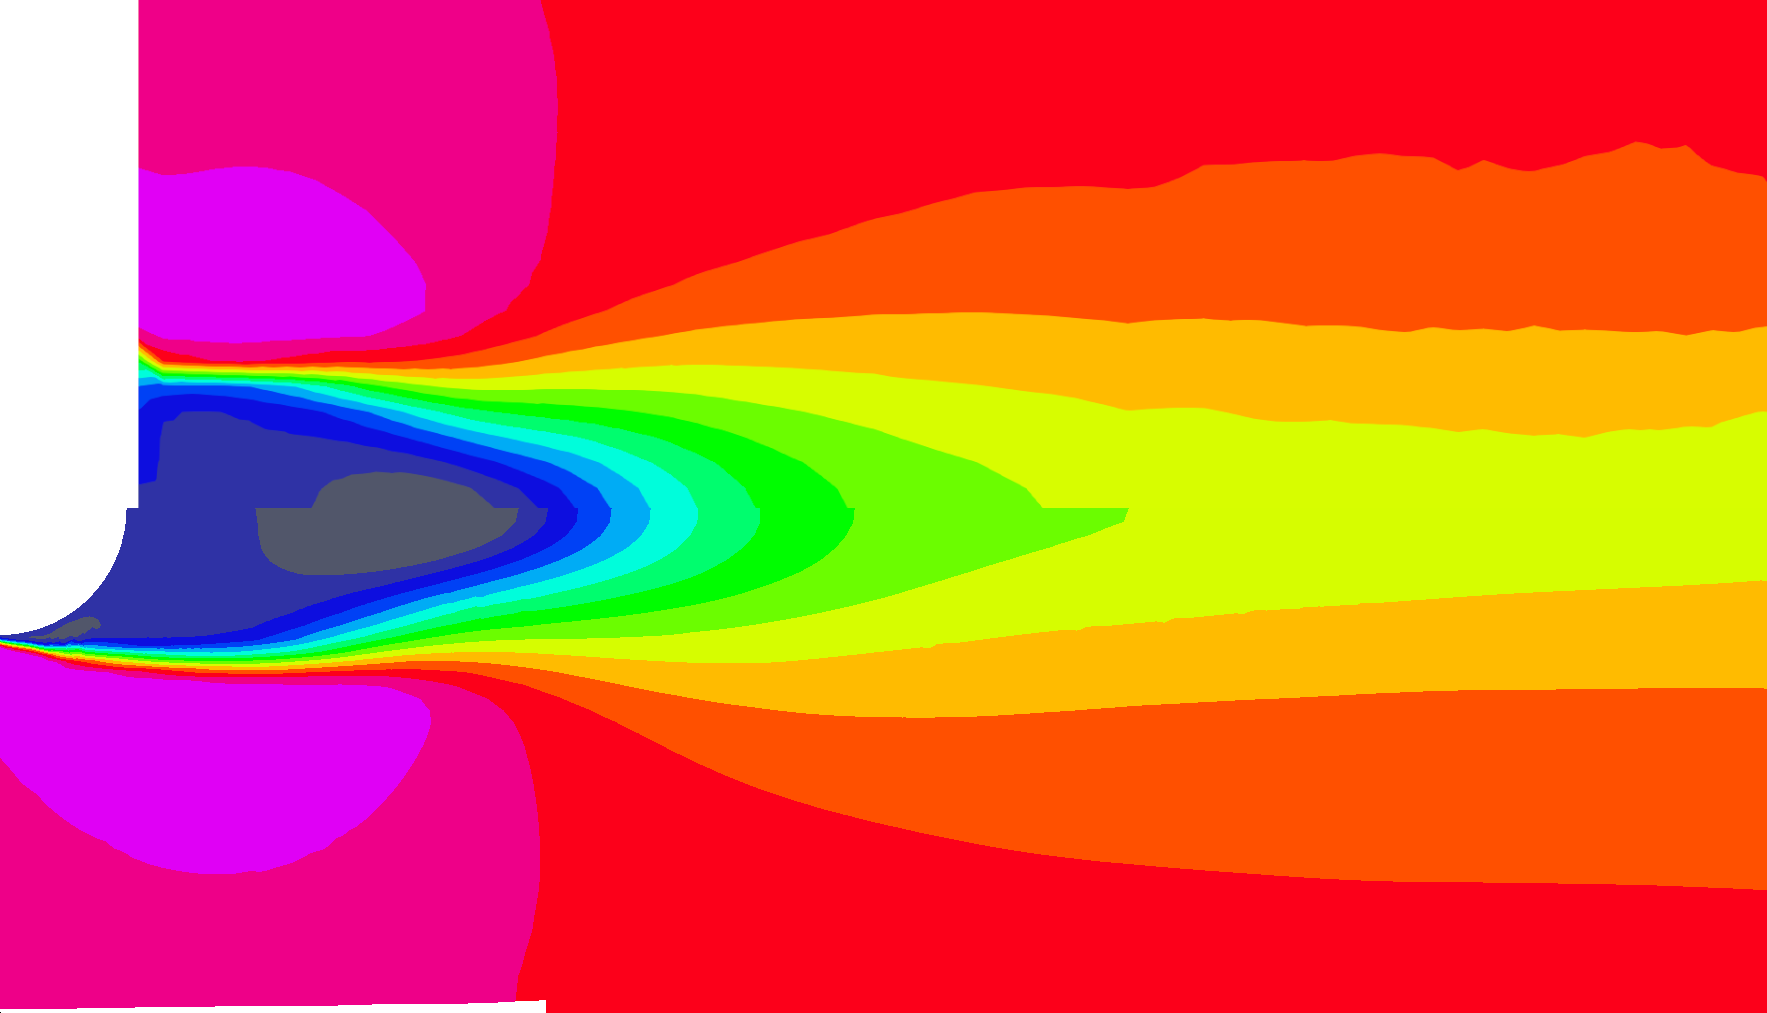
\includegraphics[trim = 0px 0px 0px 0px,clip,width = 0.39\textwidth]{\myImages/res/uXMeanComp.png}}
	\begin{axis}[
		name = plot1,
		xlabel={$x_r$ [--]},
		ylabel={$y_r$ [--]},
		font = \scriptsize,
		xtick distance=1,ytick distance=1,
		width=\wd\mygraphic,
		height=\ht\mygraphic, %height= 5/3*0.5
		enlargelimits=false,
		scale only axis=true,
		tick align=outside,
		% x label style = {at={(axis cs:3.5,-2.7)}},
		y label style = {at={(axis cs:-1,0)}},
		ytick pos=left,
		xtick pos=top,
		line width = 1.7pt,
		]
		\addplot graphics[xmin=0, xmax=7, ymin=-2, ymax=2,includegraphics={trim = 0px 0px 0px 0px,clip}] {\myImages/res/uXMeanComp.png};
		\fill [white] (axis cs:0.001,-1.997) rectangle (axis cs:0.5,1.997);
		\fill [black!70](axis cs:0,0) circle [radius=0.5];
		\draw [black,dashdotted,line width = 1pt] (axis cs:0,0) -- (axis cs:7,0);
		\node at (axis cs:6.5,1.7) {\scriptsize{PIV}};
		\node at (axis cs:6.5,-1.7) {\scriptsize{CFD}};
		\draw [black!70,dashed,line width = 1pt] (axis cs:3.83,2) -- (axis cs:3.83,-2);
		\node [black!70] at (axis cs:4.1,1.7) {\scriptsize{$\zeta$}};
		\node  at (axis cs:6.7,0.3) {\scriptsize{$\sigma$}};
		\fill [black](axis cs:4,0) circle [radius=0.1];
		\node  at (axis cs:4.2,-0.3) {\scriptsize{$p_{1}$}};
		\fill [black](axis cs:4.53,1.15) circle [radius=0.1];
		\node  at (axis cs:5,1.15) {\scriptsize{$p_{2}$}};
		\node  at (axis cs:0.25,1.7) {\scriptsize{a)}};
	\end{axis}


	\node [name = osaUx,anchor = south east,at={(plot1.south east)},yshift=-0.7cm] {
\includegraphics[width=0.26\textwidth]{\myImages/res/U_x_scale.png}};
	\node [name = ux, anchor = east,at={(osaUx.north west)},yshift=-0.1cm,xshift=-0.1cm] {\scriptsize{$u_r$ [--]}};
	\node [name = psi0, anchor = south,at={(osaUx.north)},yshift=-0.2cm,xshift=-1.61cm] {\scriptsize{-0.2}};
	\node [name = psi0, anchor = west,at={(psi0.east)},xshift=0.22cm] {\scriptsize{0.2}};
	\node [name = psi0, anchor = west,at={(psi0.east)},xshift=0.228cm] {\scriptsize{0.6}};
	\node [name = psi0, anchor = west,at={(psi0.east)},xshift=0.228cm] {\scriptsize{1.0}};
	\node [name = psi0, anchor = west,at={(psi0.east)},xshift=0.02cm] {\scriptsize{1.3}};
	% \node [name = psiM05, anchor = north west,at={(osaPsix.south west)},yshift=0.2cm] {\scriptsize{-0.1 \%}};
	% \node [name = psiM05, anchor = north east,at={(osaPsix.south east)},yshift=0.2cm] {\scriptsize{0.1 \%}};

	\savebox\mygraphic{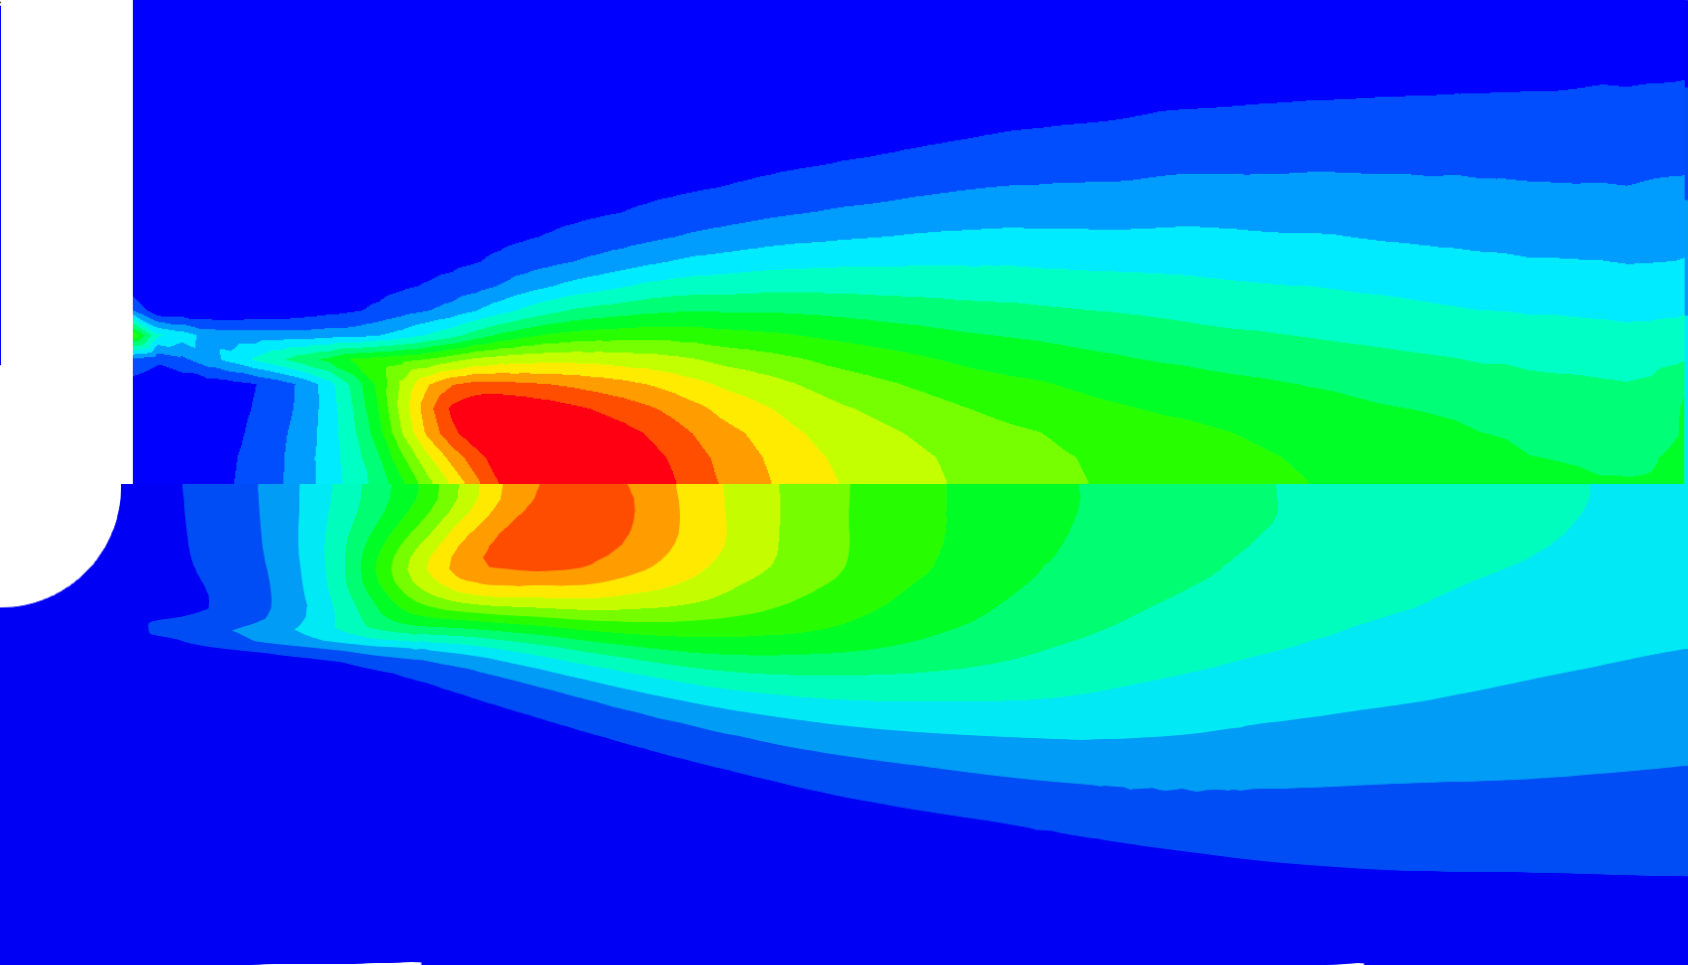
\includegraphics[trim = 0px 0px 0px 0px,clip,width = 0.39\textwidth]{\myImages/res/kMeanCompV2.png}}
	\begin{axis}[
		name = plot2,
		anchor = west,
		at = {(plot1.east)},
		xshift = 0.3cm,
		xlabel={$x_r$ [--]},
		ylabel={$y_r$ [--]},
		% x label style = {at={(axis cs:3.5,-2.7)}},
		y label style = {at={(axis cs:7.8,0)}},
		font = \scriptsize,
		xtick distance=1,ytick distance=1,
		width=\wd\mygraphic,
		height=\ht\mygraphic, %height= 5/3*0.5
		enlargelimits=false,
		scale only axis=true,
		ytick pos=right,
		xtick pos=top,
		tick align=outside,
		line width = 1.7pt,
		]
		\addplot graphics[xmin=0, xmax=7, ymin=-2, ymax=2,includegraphics={trim = 0px 0px 0px 0px,clip}] {\myImages/res/kMeanCompV2.png};
		\fill [white] (axis cs:0.001,-1.997) rectangle (axis cs:0.5,1.997);
		\fill [black!70](axis cs:0,0) circle [radius=0.5];
		\draw [black,dashdotted,line width = 1.0pt] (axis cs:0,0) -- (axis cs:7,0);
		\node  at (axis cs:6.7,0.3) {\scriptsize{$\sigma$}};
		\node [color=white] at (axis cs:6.5,1.7) {\scriptsize{PIV}};
		\node [color=white] at (axis cs:6.5,-1.7) {\scriptsize{CFD}};
		\node  at (axis cs:0.25,1.7) {\scriptsize{b)}};
	\end{axis}

	\node [name = osak,anchor = south east,at={(plot2.south east)},yshift=-0.7cm,xshift=-0.1cm] {
\includegraphics[width=0.26\textwidth]{\myImages/res/k_scale.png}};
	\node [name = k, anchor = east,at={(osak.north west)},yshift=-0.1cm,xshift=-0.1cm] {\scriptsize{$k$ [--]}};
	\node [name = psi0, anchor = south,at={(osak.north)},yshift=-0.2cm,xshift=-1.49cm] {\scriptsize{0.00}};
	\node [name = psi0, anchor = west,at={(psi0.east)},xshift=-0.085cm] {\scriptsize{0.06}};
	\node [name = psi0, anchor = west,at={(psi0.east)},xshift=-0.08cm] {\scriptsize{0.12}};
	\node [name = psi0, anchor = west,at={(psi0.east)},xshift=-0.08cm] {\scriptsize{0.18}};
	\node [name = psi0, anchor = west,at={(psi0.east)},xshift=-0.15cm] {\scriptsize{0.24}};
	\node [name = psi0, anchor = west,at={(psi0.east)},xshift=-0.2cm] {\scriptsize{0.28}};
	% \node [name = psi0, anchor = west,at={(psi0.east)},xshift=0.06cm] {\scriptsize{}};
	% \node [name = psi0, anchor = west,at={(psi0.east)},xshift=0.06cm] {\scriptsize{0.6}};
	% \node [name = psi0, anchor = west,at={(psi0.east)},xshift=0.06cm] {\scriptsize{0.6}};
	% \node [name = psi0, anchor = west,at={(psi0.east)},xshift=0.228cm] {\scriptsize{0.6}};
	% \node [name = psi0, anchor = west,at={(psi0.east)},xshift=0.228cm] {\scriptsize{1.0}};
	% \node [name = psi0, anchor = west,at={(psi0.east)},xshift=0.02cm] {\scriptsize{1.3}};

	\begin{axis}[
		width=0.805\linewidth,
		height = 3cm,
		scale only axis,
		name=plot3,
		anchor = north west,
		at = {(plot1.south west)},
		yshift = -0.8cm,
		xlabel=$x_{r,\sigma}$,
		ylabel={$u_r$ [--]},
		%~ ymode=log,
		%~ xmode=log,
		ymax = 0.8,
		xmin = 0.5,
		ymin = -0.5,
		xmax = 7,
		ytick pos=left,
		font = \scriptsize,
		mark size=4pt,    
		line width = 0.85pt,
		%~ legend style={at={(axis cs:6,2)},anchor=south west},				
	]
	\addplot [color = black,mark =none]table [y=u_x,x =x]{\myGraphs/msIndData/expLineResV1.dat};\label{ux_sigma}
	\addplot [color = red,mark =none]table [y=u_x,x =x]{\myGraphs/msIndData/expLineResV1.dat};\label{expSigm}
	% \addplot [color = blue,mark =none]table [col sep=comma, y expr=(\thisrow{U:0})/5,x expr = {(\thisrow{Points:0})/0.015}]{\myGraphs/msIndData/mS_40p_U.csv};\label{mesh40U}
	% \addplot [color = red,mark =none]table [col sep=comma, y expr=(\thisrow{U:0})/5,x expr = {(\thisrow{Points:0})/0.015}]{\myGraphs/msIndData/mS_50p_U.csv};\label{mesh50U}
	% \addplot [color = green,mark =none]table [col sep=comma, y expr=(\thisrow{U:0})/5,x expr = {(\thisrow{Points:0})/0.015}]{\myGraphs/msIndData/mS_75p_U.csv};\label{mesh70U}
	\addplot [color = blue,mark =none]table [col sep=comma, y expr=(\thisrow{U:0})/5,x expr = {(\thisrow{Points:0})/0.015}]{\myGraphs/msIndData/bCyl_l_3_U.csv};\label{numSigm}
	% \addplot [color = blue,mark =none]table [col sep=comma, y expr=(\thisrow{U:0})/5,x expr = {(\thisrow{Points:0})/0.015}]{\myGraphs/msIndData/u_xprofPOM1.csv};\label{numSigm}
	% \addplot [color = orange,mark =none]table [col sep=comma, y expr=(\thisrow{U:0})/5,x expr = {(\thisrow{Points:0})/0.015}]{\myGraphs/msIndData/mS_120p_U.csv};\label{mesh120U}
	%~ \addplot [color = red,mark =none]table [y=U_x_ms_50_U,x =z_ms_50_U]{\myGraphs/onLineMSV2.dat};\label{mesh50U}
	%~ \addplot [color = green,mark =none]table [y=U_x_ms_70_U,x =z_ms_70_U]{\myGraphs/onLineMSV2.dat};\label{mesh70U}
	%~ \addplot [color = black,mark =none]table [y=U_x_ms_100_U,x =z_ms_100_U]{\myGraphs/onLineMSV2.dat};\label{mesh100U}
	%~ \addplot [color = black,mark =none]table [y=U_x_ms_100_U,x =z_ms_120_U]{\myGraphs/onLineMSV2.dat};\label{mesh100U}
	\coordinate (top) at (rel axis cs:0,1);
	\node  at (axis cs:0.7,0.65) {\scriptsize{c)}};
	\end{axis}
\begin{axis}[
		at = (plot3.north west),
		anchor = north west,
		width=0.805\linewidth,
		height = 3cm,
		scale only axis,
		xlabel=$x_\sigma$,
		%~ ylabel={\textcolor{red}{TKE}},
		ylabel={$k$ [--]},
		%~height=\figHeight,
		scale only axis,
		font = \scriptsize,
		%~ xmin=0,
		%~ xmax=600,
		xmin=0.5,
		xmax=7,
		ymin=0,
		ymax = 0.3,
		%~ ymax=1000,
		hide x axis,
		axis y line*=right,
		line width = 0.85pt,
		%~ axis line style={red},
		%~ axis y label/.append style ={red},
		%~ ytick label/.append style = {red},
		%~ ylabel={$y_{\mathrm{NO}},\,y_{\mathrm{N_{2}O}} \mathrm{\,[ppm]}$},
		mark size=2.5pt, 
	]
	\addplot [color = black,mark =none,dashed]table [y=k,x =x]{\myGraphs/msIndData/expLineResKV1.dat};\label{k_sigma}
	\addplot [color = red,mark =none,dashed]table [y=k,x =x]{\myGraphs/msIndData/expLineResKV1.dat};
	% \addplot [color = blue,mark =none,dashed]table [col sep=comma, y expr=(\thisrow{k}),x expr = {(\thisrow{Points:0})/0.015}]{\myGraphs/msIndData/mS_40p_k.csv};\label{mesh40k}
	% \addplot [color = red,mark =none,dashed]table [col sep=comma, y expr=(\thisrow{k}),x expr = {(\thisrow{Points:0})/0.015}]{\myGraphs/msIndData/mS_50p_k.csv};\label{mesh50k}
	% \addplot [color = green,mark =none,dashed]table [col sep=comma, y expr=(\thisrow{k}),x expr = {(\thisrow{Points:0})/0.015}]{\myGraphs/msIndData/mS_75p_k.csv};\label{mesh70k}
	% \addplot [color = blue,mark =none,dashed]table [col sep=comma, y expr=(\thisrow{k}),x expr = {(\thisrow{Points:0})/0.015}]{\myGraphs/msIndData/bCyl_l_3_k.csv};
	\addplot [color = blue,mark =none,dashed]table [col sep=comma, y expr=(\thisrow{"k"}),x expr = {(\thisrow{"Points:0"})/0.015}]{\myGraphs/msIndData/Znorm_kMean.csv};
	% \addplot [color = orange,mark =none,dashed]table [col sep=comma, y expr=(\thisrow{k}),x expr = {(\thisrow{Points:0})/0.015}]{\myGraphs/msIndData/mS_120p_k.csv};\label{mesh120k}

	\coordinate (bot) at (rel axis cs:1,0);
\end{axis}

\matrix[
	matrix of nodes,
	anchor=north east,
	draw,
	inner sep=0.2em,
	font = \scriptsize,
	%~ thick,
	fill=white,
  ]at([xshift=-0.2cm,yshift=-0.4cm]plot3.north east)
  {
	%~ \ref{100}& CFD old &[5pt]\\
	%~ \ref{60}& XPF - reac, wall&[5pt]\\
	\ref{expSigm}& PIV &
	% \ref{mesh40U}& 40 U &
	% \ref{uxExp}& $U$ exp &[5pt]\\
	% \ref{mesh50U}& 50 U &
	% \ref{mesh70U}& 75 U &
	\ref{ux_sigma}& $u_{r}$ &
	% \ref{mesh120U}& 120 U
	\\
	\ref{numSigm}& CFD &
	% \ref{mesh40k}& 40 k &
	% \ref{uxExp}& $U$ exp &[5pt]\\
	% \ref{mesh50k}& 50 k &
	% \ref{mesh70k}& 75 k &
	\ref{k_sigma}& $k$ &
	% \ref{mesh120k}& 120 k
	\\
%        \ref{legendNoReact}& $\mathrm{thermic\ no\ reaction\ heat}$&[5pt]
	\\};
\end{tikzpicture}